% Homework report template for courses lectured by Blaz Zupan.
% For more on LaTeX please consult its documentation pages, or
% read tutorials like http://tobi.oetiker.ch/lshort/lshort.pdf.
%
% Use pdflatex to produce a PDF of a report.

\documentclass[a4paper,11pt]{article}
\usepackage[slovene]{babel}
\usepackage{a4wide}
\usepackage{fullpage}
\usepackage[toc,page]{appendix}
\usepackage[pdftex]{graphicx} % for figures
\usepackage{setspace}
\usepackage{color}
\definecolor{light-gray}{gray}{0.95}
\usepackage{listings} % for inclusion of Python code
%\usepackage[colorlinks=false]{hyperref}
%\usepackage[hidelinks]{hyperref}
%\usepackage{hyperref}
\usepackage[bookmarks=true,pdfborder={0 0 0}]{hyperref}
\renewcommand{\baselinestretch}{1.2}

\setlength{\parindent}{0pt}

\lstset{ % style for Python code, improve if needed
    language=Python,
    basicstyle=\footnotesize,
    basicstyle=\ttfamily\footnotesize\setstretch{1},
    backgroundcolor=\color{light-gray},
}

\title{Modeliranje brez\v{z}i\v{c}nih omre\v{z}ij}
\author{
    Maja Podbevšek\\
    Peter Benko (63090004)\\
    \v{Z}iga Ham\\
    Miha Zidar (63060317)
}
\date{\today}

\begin{document}

\maketitle

\pagebreak

\tableofcontents

\pagebreak

\section{Zgledi}


%%%%%%%%%%%%%%%%%%%%%%%%%%%%%%%%%%%%%%%%%%%%%%%%%%%%%%%%%%%%%%%%%%%%%%%%%%%%

\subsection{HandOver}

V zgledu imamo naslednje module (Slika \ref{image:handover}):

\begin{itemize}
    \item dve dostopni točki
    \item enega odjemalca
    \item modul Configurator
\end{itemize}

Imamo le eno možno konfiguracijo. Odjemalec se premika po prostoru in na določeni točki zamenja dostopno točko s katero komunicira. 

\begin{figure}[htbp]
    \begin{center}
        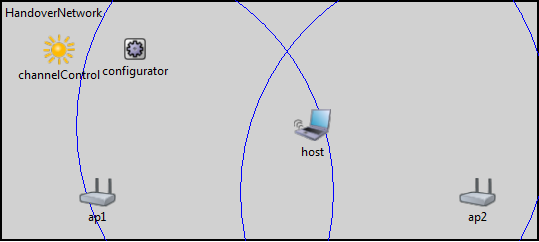
\includegraphics[scale=0.8]{img/zgledi/handover.png}
        \caption{Zgled HandOver}
        \label{image:handover}
    \end{center}
\end{figure}

%%%%%%%%%%%%%%%%%%%%%%%%%%%%%%%%%%%% HostToHost %%%%%%%%%%%%%%%%%%%%%%%%%%%%%%%%%%%%%%%%

\subsection{HostToHost}
V zgledu imamo naslednje module :

\begin{itemize}
    \item nekaj odjemalcev, od katerih en deluje kot strežnik
    \item eno dostopno točko
\end{itemize}

Odjemalec in strežnik sta povezana z brezžično povezavo.\\

Na razpolago imamo dve možni konfiguraciji:

\begin{itemize}
    \item Throughput1 (Slika \ref{image:hosttohost}) – 6 odjemalcev in en strežnik skozi dostopno točko
    \item General (Slika \ref{image:hosttohostgeneral}) – poljubno število odjemalcev in en strežnik skozi dostopno točko
\end{itemize}

Z zgledom merimo prepustnost omrežja pri komunikaciji odjemalca s strežnikom. Opazujemo tudi vpliv ostalih odjemalcev na komunikacijo med zgoraj omenjenim odjemalcem in strežnikom. Vsi akterji v omrežju povzročajo šum in s tem zmanjšujejo prepustnost.


\begin{figure}[htbp]
    \begin{center}
        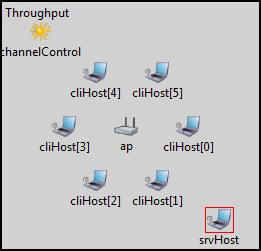
\includegraphics[scale=0.8]{img/zgledi/hosttohost.png}
        \caption{Zgled HostToHost, s konfiguracijo Throughput1}
        \label{image:hosttohost}
    \end{center}
\end{figure}

\begin{figure}[htbp]
    \begin{center}
        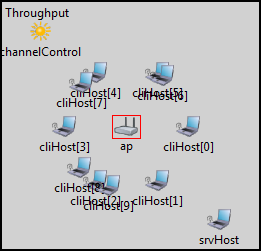
\includegraphics[scale=0.8]{img/zgledi/hostohost_general.png}
        \caption{Zgled HostToHost, s konfiguracijo General}
        \label{image:hosttohostgeneral}
    \end{center}
\end{figure}

%%%%%%%%%%%%%%%%%%%%%%%%%%%%%%%%%%%% MultiRadio %%%%%%%%%%%%%%%%%%%%%%%%%%%%%%%%%%%%%%%%

\subsection{MultiRadio}

V zgledu imamo naslednje module:

\begin{itemize}
    \item dva odjemalca
    \item dve dostopni točki
    \item en usmerjevalnik
    \item modul Configurator
\end{itemize}

Imamo tri konfiguracije:

\begin{itemize}
    \item Switched Wlans (Slika \ref{image:multiradioswitched}) – povezava dostopnih točk preko ethernet stikala
    \item Routed Wlans (Slika \ref{image:multiradiorouted}) – dva WLAN-a povezana preko usmerjevalnika z dvema brezžičnima mrežnima karticama
    \item Independent Wlans (Slika \ref{image:multiradioindependent}) – dva neodvisna WLAN-a na različnih radijskih kanalih
    \item General (Slika \ref{image:multiradiogeneral}) – dva neodvisna WLAN-a preko usmerjevalnika
\end{itemize}

Zgled prikazuje uporabo večih brezžičnih vmesnikov na enem usmerjevalniku, tako da imamo več brezžičnih omrežij na različnih kanalih.


\begin{figure}[htbp]
    \begin{center}
        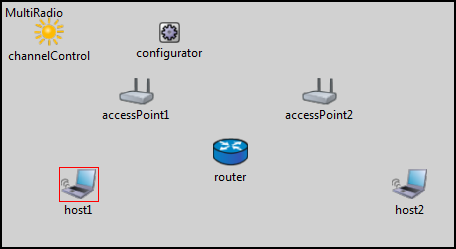
\includegraphics[scale=0.8]{img/zgledi/multiradio_general.png}
        \label{image:multiradiogeneral}
        \caption{Zgled MultiRadio, s konfiguracijo General}
    \end{center}
\end{figure}

\begin{figure}[htbp]
    \begin{center}
        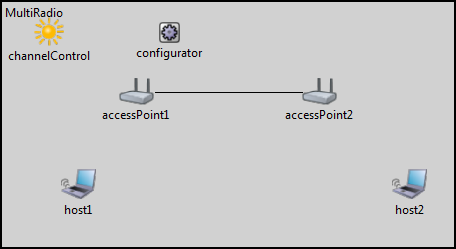
\includegraphics[scale=0.8]{img/zgledi/multiradio_switched.png}
        \caption{Zgled MultiRadio, s konfiguracijo Switched Wlans}
        \label{image:multiradioswitched}
    \end{center}
\end{figure}

\begin{figure}[htbp]
    \begin{center}
        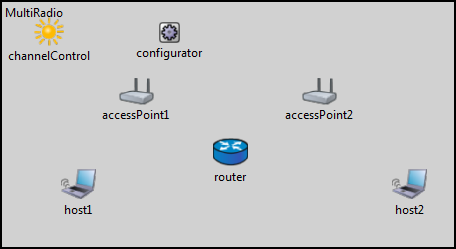
\includegraphics[scale=0.8]{img/zgledi/multiradio_routed.png}
        \caption{Zgled MultiRadio, s konfiguracijo Routed Wlans}
        \label{image:multiradiorouted}
    \end{center}
\end{figure}

\begin{figure}[htbp]
    \begin{center}
        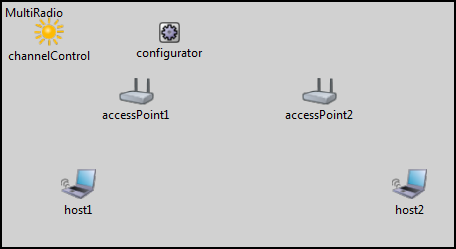
\includegraphics[scale=0.8]{img/zgledi/multiradio_independent.png}
        \caption{Zgled MultiRadio, s konfiguracijo Independent Wlans}
	\label{image:multiradioindependent}
    \end{center}
\end{figure}

%%%%%%%%%%%%%%%%%%%%%%%%%%%%%%%%%%%% Synchronized %%%%%%%%%%%%%%%%%%%%%%%%%%%%%%%%%%%%%%%%

\subsection{Synchronized}

V zgledu imamo naslednje module:
\begin{itemize}
    \item AdhocHost
    \item modul Configurator
\end{itemize}

V zgledu opazujemo anomalije pri generiranju brezžičnega prometa, ki jih povzroča sinhrono pošiljanje paketov.

Imamo dve konfiguraciji (Slika \ref{image:synchronized}):
\begin{itemize}
    \item Synchronized – sinhrono pošiljanje paketov, pri katerem prihaja do kolizij, ki so posledica istočasnega oddajnja paketov, zato sporočila niso sprejeta.
    \item NonSynchronized – nesinhrono pošiljanje paketov, kolizij je občutno manj, saj vplejemo naključni časovni zamik pri pošiljanju paketov.
\end{itemize}


\begin{figure}[htbp]
    \begin{center}
        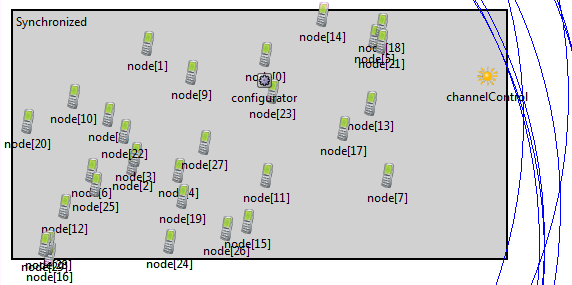
\includegraphics[scale=0.8]{img/zgledi/synchronized_sync.png}
        \caption{Zgled Synchronized, s sinhrono in asinhrono konfiguracijo}
	\label{image:synchronized}
    \end{center}
\end{figure}



%%%%%%%%%%%%%%%%%%%%%%%%%%%%%%%%%%%% Throughput %%%%%%%%%%%%%%%%%%%%%%%%%%%%%%%%%%%%%%%%

\subsection{Throughput}

V zgledu imamo naslednje module:
\begin{itemize}
    \item nekaj mobilnih odjemalcev
    \item eno dostopno točko
\end{itemize}

Z zgeldom merimo prepustnost omrežja med večinimi odjemalci in dostopno točko. Prepustnost je vedno manjša od teoretične maksimalne, saj si odjemalci delijo medij in prihaja do kolizij. Odjemalci in dostopna točka so konfigurirani tako, da vsak odjemalec sliši vse ostale odjemalce.\\

Imamo dva ničina konfiguracije:

\begin{itemize}
    \item Throughput1 (Slika \ref{image:throughputthr1}) – en odjemalec do dostopne točke
    \item Throughput2 (Slika \ref{image:throughputthr2}) – trije odjemalci do dostopne točke
    \item General (Slika \ref{image:throughputgeneral}) – poljubno število odjemalcev do dostopne točke
\end{itemize}

Prepustnost merimo s ``Sink'' podmodulom dostopne točke.

Vsi zgledi vsebujejo tudi modul ChannelControl. Moduli so podrobno opisani v analizi zgleda Lan80211.


\begin{figure}[htbp]
    \begin{center}
        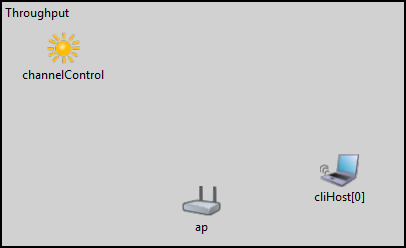
\includegraphics[scale=0.8]{img/zgledi/throughput_thr1.png}
        \caption{Zgled Throughput, s konfiguracijo Throughput1}
	\label{image:throughputthr1}
    \end{center}
\end{figure}


\begin{figure}[htbp]
    \begin{center}
        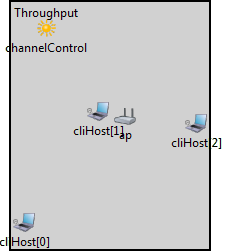
\includegraphics[scale=0.8]{img/zgledi/throughput_thr2.png}
        \caption{Zgled Throughput, s konfiguracijo Throughput2}
	\label{image:throughputthr2}
    \end{center}
\end{figure}

\begin{figure}[htbp]
    \begin{center}
        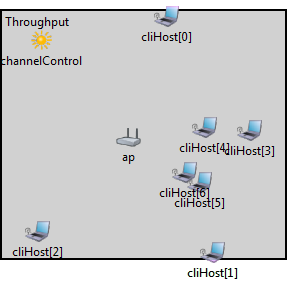
\includegraphics[scale=0.8]{img/zgledi/throughput_general.png}
        \caption{Zgled Throughput, s konfiguracijo General}
	\label{image:throughputgeneral}
    \end{center}
\end{figure}



%%%%%%%%%%%%%%%%%%%%%%%%%%%%%%%%%%%% 80211 %%%%%%%%%%%%%%%%%%%%%%%%%%%%%%%%%%%%%%%%


\section{Lan80211}


\begin{figure}[htbp]
    \begin{center}
        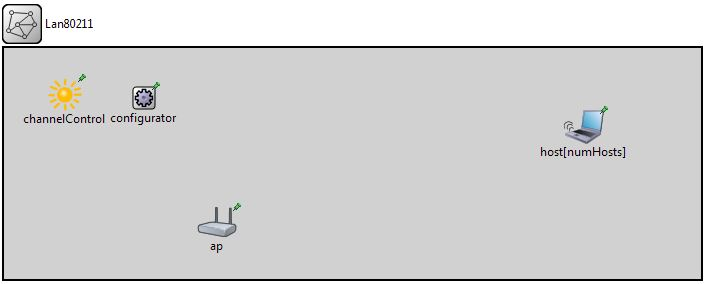
\includegraphics[scale=0.8]{img/lan80211.jpg}
        \caption{Shema modela 802.11}
	\label{image:lan80211}
    \end{center}
\end{figure}


\subsection{Gradniki}

\subsubsection{Access Point}
\label{description:acceesspoint}

oziroma dostopna točka je enota, ki lahko sprejema in oddaja brezžične signale. Hrani tudi tabelo vseh enot, ki so trenutno povezana na njo. Ima ena žična vrata v svetovni splet, ter na drugi strani anteno za brezžično komunikacijo. Vmes podatke posreduje relacijska enota. 

\begin{figure}[htbp]
    \begin{center}
        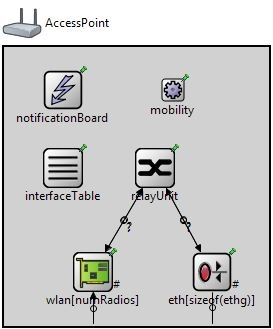
\includegraphics[scale=0.8]{img/ap.jpg}
        \caption{Shema dostopne točke}
	\label{image:ap}
    \end{center}
\end{figure}


\paragraph{interfaceTable}
\label{description:interfaceTable}

je objekt preprostega modula InterfaceTable. Nima nikakeršnih vrat in posledično tudi ne obdelave sporočil. Uporablja se zgolj z uporabo funkcij. Deluje kot slovar za prevajanje, ali še bole, kot tabela za prevajanje vseh priključenih naprav. Obdeluje se dinamično, ob priklopu se nova naprava registrira v tabelo in poskrbi za vnose v routing tabele (IRoutingTable in IRoutingTable6). V interfaceTable se vnašajo InterfaceEntry-ji, ki vsebujejo podatke, kot so: interfaceId(unikadtna identifikacijska številka, ki zaznamuje vnos), id vhodnih in izhodnih vrat naslovnika, MTU, pasovno širino, MAC naslov, trenutno stanje (up/down) ter podatke kaj podpira (broadcast, multicast, point to point, loopback).



\paragraph{notificationBoard}
\label{description:notificationBoard}

je objekt preprostega mudula ``notificationBoard'', s katerim realiziramo vmesnik za sprejemanje in zazpečevanje obvestil. ob prijavise v tem modulu vsak odjemalec ``prijavi'' na kategorije, ki se jih tičejo. Če želi katerikoli od odjemalcev poslati sporočilo mora zahtevo najprej predati notificationBoard-u, ki potem razpošlje tosporočilo vsem primernim odjemalcem, torej takim, ki so naročeni na specifično ``kategorijo''.

\paragraph{wlan[]}
\label{description:wlan}

predstavlja brezžično mrežno kartico (IWirelessNic - Wireless Network Interface Controller, po protokolu implementiranem v Ieee80211Nic), ki je razširitev modula mrežnih kartic ('INic'). Gre za eno kartico, na kateri vsak vnos v tabelo wlan[] predstavlja eno anteno oz. oddajnik. Vsebovani moduli so prikazani na Sliki \ref{image:radio} (modul Ieee80211Radio) je fizični nivo wlan-a. Oddaja in sprejema brezžične signale ter jih posreduje enoti 'mac' (modul Ieee80211Mac). Mac za sprejeti paket skrbi, da se je pravilno sprejel, oz. da se bo pravilno poslal. Pri pošiljanju potrebuje vsa polja paketa izpolnjena. Sam zna zapolniti le izvorni MAC naslov paketka. Enota mgmt (modul IIeee80211Mgmt) posreduje pakete med nivoji ter dodaja funkcionalnost agenta. Agent (preprost modul Ieee80211AgentSTA) skrbi za skeniranje kanalov, antentikacijo ter povezovanje. Deluje v dveh načinih skeniranja: aktivno ter pasivno. Agentu (modul Ieee80211AgentSTA) lahko podamo spisek kanalov, ki naj jih preveri, zamik med skeniranji, minimalni čakalni čas, ki ga mora porabiti na določenem kanalu med aktivnim skeniranjem, čas ki ga porabi na vsakemkanalu ob pasivnem skeniranju, avtentikacijski timeout ter timeout za povezovanje. Agentu določa tudi SSID, ki ga bo wlan[] oglaševal. Input in output zanki sta realizirani zgolj za simulacijo, saj sta zelo primerni za umetno ustvarjanje določenih napak na omrežju.


\begin{figure}[htbp]
    \begin{center}
        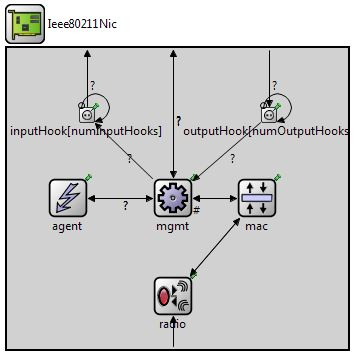
\includegraphics[scale=0.8]{img/radio.jpg}
        \caption{Shema dostopne točke}
	\label{image:radio}
    \end{center}
\end{figure}


\paragraph{relayUnit}
\label{description:relayUnit}


\paragraph{eth[]}
\label{description:eth}


\end{document}

